\chapter{Présentation de Mobigis}
\label{PresentationEntreprise}

\section{Domaine d'application}\label{sig}

Les Systèmes d'Informations Géographiques (SIG) sont des outils informatiques permettant de représenter et d'analyser toutes les choses qui existent sur terre ainsi que tous les événements qui s'y produisent.
Les SIG offrent toutes les possibilités des bases de données (telles que requêtes et analyses statistiques) et ce, au travers d'une visualisation unique et d'analyse géographique propres aux cartes. Ces capacités spécifiques font du SIG un outil unique, accessible à un public très large et s'adressant à une très grande variété d'applications. 
Les enjeux majeurs auxquels nous avons à faire face aujourd'hui (environnement, démographie, santé publique…) ont tous un lien étroit avec la géographie. De nombreux autres domaines tels que la recherche et le développement de nouveaux marchés, l'étude d'impact d'une construction, l'organisation du territoire, la gestion de réseaux, le suivi en temps réel de véhicules, la protection civile… sont aussi directement concernés par la puissance des SIG pour créer des cartes, pour intégrer tout type d'information, pour mieux visualiser les différents scénarios, pour mieux présenter les idées et pour mieux appréhender l'étendue des solutions possibles.
Les SIG sont utilisés par tous ; collectivités territoriales, secteur public, entreprise, écoles, administrations, états utilisent les SIG. La création de cartes et l'analyse géographique ne sont pas des procédés nouveaux, mais les SIG procurent une plus grande vitesse et proposent des outils sans cesse innovant dans l'analyse, la compréhension et la résolution des problèmes.
L'avènement des SIG a également permis un accès à l'information à un public beaucoup plus large (ex : Google Maps). Aujourd'hui, les SIG représentent un marché de plusieurs milliards d'euros dans le monde et emploient plusieurs centaines de milliers de personnes. 
Le SIG appliqué aux transports, peut être utilisé pour gérer et analyser certaines informations essentielles :
\begin{itemize}
\item Planification et modélisation des transports
\item Planification et analyse des itinéraires 
\item Localisation et suivi automatiques des véhicules 
\item Inventaire des arrêts de bus et des infrastructures, gestion des installations ferrées 
\item etc. 
\end{itemize}

\section{Présentation de l'entreprise}

MobiGIS\footnote{site de l'entreprise \url{http://www.mobigis.fr/}} se présente comme une entreprise au coeur de l'innovation, dont l'activité est d'apporter des réponses sur-mesure aux besoins de ses clients en matière de \textbf{géomatique}, notamment lorsqu'elle est appliquée aux enjeux de transport et de mobilité. MobiGIS est une société innovante éditrice de solutions dans le domaine des Systèmes d'Information Géographique (SIG). 
Elle intervient dans les thématiques : de l'environnement et du développement durable ; de la mobilité des personnes ; du transport et de la logistique (Fig. \ref{OffresMobigis}).\\

Ses équipes font de la conception, mise en \oe uvre et déploiement d'architectures SIG, développement d'applications de cartographie web et mobiles, études de transports, solutions de prévention des risques, etc. L'entreprise est compétente dans l'édition de logiciels SIG, le conseil et les services en SIG, la R\&D liée aux NTIC\footnote{exemples de réalisations \url{http://www.mobigis.fr/realisations/}}.\\

\begin{center}
\begin{figure}[h] \centering
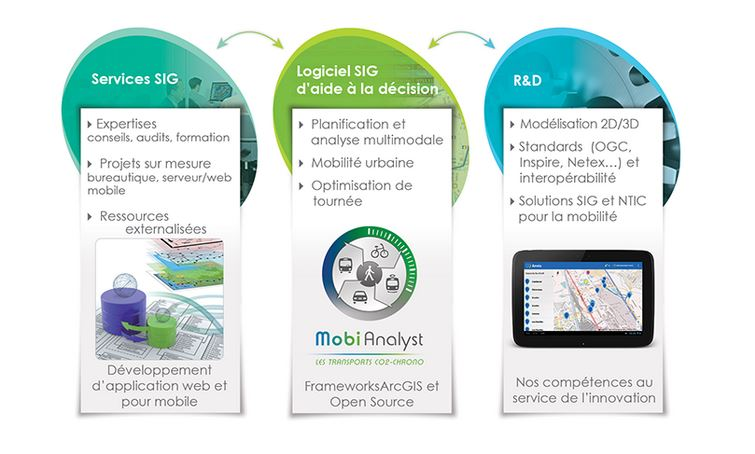
\includegraphics[width=16cm]{images/fig1_solutionsMobigis.JPG}\\
\caption{\label{OffresMobigis} Offres de services Mobigis}
\end{figure}
\end{center}


\pagebreak

\section{Activités}

L'activité de MobiGIS est centrée sur les services SIG et l'édition de logiciels. Les clients de MobiGIS sont par exemples des industries, la grande distribution, les collectivités locales, et les intégrateurs et société de services en ingénierie informatique (SSII) (Fig. \ref{ClientsMobigis}). L'entreprise développe en particulier une activité d'édition de logiciels. Ceux-ci permettent de faire des analyses multiples : territoire, pollutions, démographie, etc., d'élaborer des plans de déplacement urbain et entreprise, d'étudier et de préparer la réorganisation des réseaux multimodaux et la création de nouvelles infrastructures de transport. Elle compte parmi ses clients des Autorités Organisatrices de Transports (ex : Tisseo), des bureaux d'études, des sociétés de consulting immobilier, des agences d'urbanisme, etc.\\

\begin{center}
\begin{figure}[h] \centering
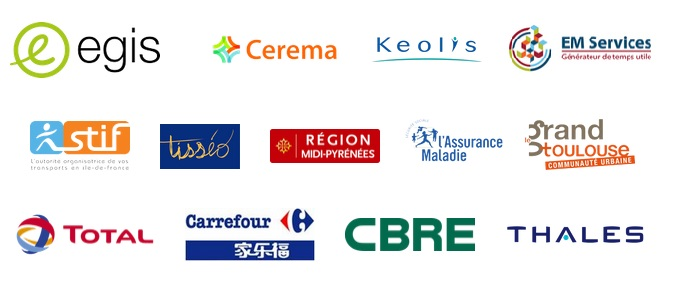
\includegraphics[width=16cm]{images/fig2_referencesMobigis.JPG}\\
\caption{\label{ClientsMobigis} Exemples de clients Mobigis}
\end{figure}
\end{center}

\section{Historique}

\renewcommand{\labelitemi}{\textbullet}
\begin{itemize}
\item 2007 
    - Création de la société MobiGIS par Frédéric SCHETTINI 
		
    - Le projet de création de société a obtenu le titre de « projet de création d'entreprises innovantes » par le pôle innovation de la Chambre de Commerce et d'Industrie de Toulouse 
		
    - La société MobiGIS est accompagnée par Oséo Midi-Pyrénées 
    
		- MobiGIS obtient le statut de Jeune Entreprise Innovante (JEI) 
\\
\item 2008 
    - Mise en place d'une démarche active de développement des activités de MobiGIS en Chine 
    
		- Obtention du Prix TOTAL de l'Innovation IT 
    
		- Phase intensive de Recherche Développement 
    
		- Début de collaboration avec le CNRS/LAAS 
    
		- Labellisation du projet POTIMART par la PREDIM 
\\
\item 2009 
    - Emménagement sur le site de Grenade-sur-Garonne (31) 
    
		- MobiGIS intègre le groupement CECILE, composé de PME Toulousaines spécialisées dans la géolocalisation 
    
		- MobiGIS rejoint l'association JEInnov 
\\
\item 2010 
    - MobiGIS accompagne le ministre des transports en Chine 
    
		- Labellisation par la Plateforme de Recherche et d'Expérimentation pour le Développement de l'Information Multimodale (PREDIM) du projet CAMERA 
    
		- MobiGIS recrute un Volontaire International en Entreprise (VIE) pour intensifier son développement en Chine 
    
		- Soutien de la Région de Midi-Pyrénées pour un Contrat d'appui 
\\
\item 2011 
    - Commercialisation du progiciel MobiAnalyst 
    
		- Soutien de la CCIT et d'HGI Tech pour intensifier son développement commercial 
    
		- Recrutement d'un chef de projets SI et d'un ingénieur commercial 
\\
\item 2012 
    - L'équipe MobiGIS s'étoffe et compte désormais plus de 10 collaborateurs 
    
		- Prix de l'innovation au Toulouse Space Show et lauréat du concours Open Data « Défi numérique Toulouse Métropole » 
    
		- Ouverture d'un bureau à Paris 
    
		- Adhésion à l'Aerospace Valley 
    
		- Participation à 10 congrès dont l'ITS World à Vienne 
\\
\item 2013 
    - Signature de nouveaux contrats avec le groupe Total, Carrefour China, et l'APEM 
    
		- Lancement de la solution Anvio et de la V2.3 de MobiAnalyst 
\\
\item 2014
    - MobiAnalyst© remporte le prix de meilleure application de l'année !
    
		- Ouverture d'un bureau au Canada pour intensifier l'activité en Amérique du Nord
    
		- Premier Workshop MobiGIS organisé en septembre 2014 

\end{itemize}



\section{Ressources de l'entreprise}

Les compétences humaines permettent à l'entreprise de mener à bien des projets SIG, l'implémentation d'architecture logicielle, de systèmes de gestion de bases de données spatiales, et enfin de développer des solutions bureautique, serveur, web et mobile. 
L'entreprise héberge également les compétences nécessaires pour mener à bien des missions de conseil, d'audit et de consulting. Elle peut établir des états des lieux, des analyses et des préconisations. Enfin, MobiGIS propose des formations sur ses progiciels sur site ou à distance. \\

Les technologies maîtrisées par MobiGIS sont les logiciels SIG propriétaires, les SIG libres, et les langages de programmation logiciel, web et mobile. Parmi les logiciels SIG propriétaires il y a en premier lieu ESRI ArcGIS\footnote{\url{http://www.esrifrance.fr/arcgis.aspx}}, mais aussi MapInfo, GeoConcept et Google Maps sont également présents. Actuellement, l'entreprise s'inscrit dans la tendance de nombreux éditeurs, de ne plus seulement proposer des solutions desktop (qui imposent d'installer des logiciels sur son poste de travail, etc...) mais aussi de proposer des solutions à distance, plus souples (et moins onéreuses pour l'acheteur), notamment sur le modèle d'ArcGIS Online\footnote{\url{http://www.esrifrance.fr/ArcGIS_Online_1.aspx}}. Les SIG libres sont aussi très présents dans les projets dont notamment les logiciels QGIS, PostGIS, OpenLayers, ou encore GeoServer. \\

Les langages "objets" maîtrisés par les développeurs et géomaticiens de l'entreprise sont divers dont notamment Java, C++, C\#, Python… Ils permettent de programmer les progiciels de l'entreprise. L'équipe MobiGIS pratique également les langages web du moment : HTML 5, JavaScript, PHP, CSS 3,etc. Ils développent sur les principaux supports mobiles : IOS et Android, qui prennent aujourd'hui une importance croissante dans le monde des SIG en raison de l'évolution des pratiques liées à l'utilisation des smartphones et des tablettes. \\